\documentclass[tikz,border=10pt]{standalone}
\usepackage{amsmath}
\usetikzlibrary{angles,quotes}

\begin{document}
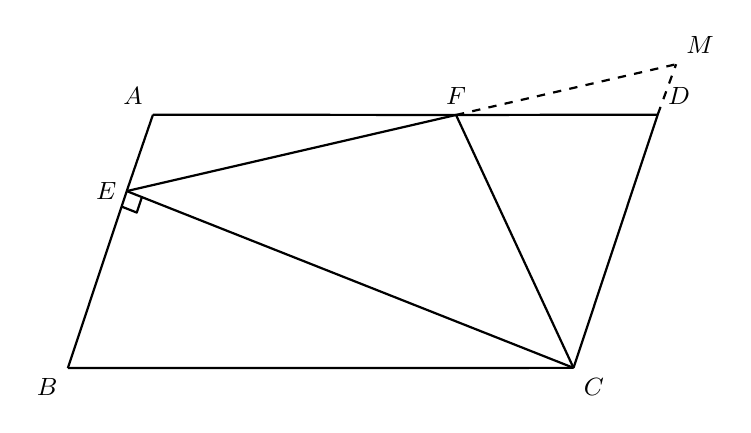
\begin{tikzpicture}[line width=0.8pt, line join=round]
\coordinate (A) at (-2.804,1.292);
\coordinate (B) at (-3.885,-1.926);
\coordinate (C) at (2.537,-1.923);
\coordinate (D) at (3.606,1.292);
\coordinate (F) at (1.045,1.289);
\coordinate (M) at (3.840,1.933);




\coordinate (E) at (-3.137,0.322);


\draw (A) -- (F);
\draw (F) -- (D);
\draw (A) -- (D);


\draw (A) -- (E) -- (B);
\draw (B) -- (C);
\draw (C) -- (D);


\draw (C) -- (F);
\draw (F) -- (E);
\draw (E) -- (C);


\draw[dashed] (F) -- (M);
\draw[dashed] (D) -- (M);


\draw pic[draw, angle radius=0.207cm] {right angle=B--E--C};


\node[font=\fontsize{9}{10.8}\selectfont, above left] at (A) {$A$};
\node[font=\fontsize{9}{10.8}\selectfont, below left] at (B) {$B$};
\node[font=\fontsize{9}{10.8}\selectfont, below right] at (C) {$C$};
\node[font=\fontsize{9}{10.8}\selectfont, above right] at (D) {$D$};
\node[font=\fontsize{9}{10.8}\selectfont, above] at (F) {$F$};
\node[font=\fontsize{9}{10.8}\selectfont, left] at (E) {$E$};
\node[font=\fontsize{9}{10.8}\selectfont, above right] at (M) {$M$};
\end{tikzpicture}
\end{document}